\documentclass[11pt, a4paper]{article}

% Fonts and Encoding
\usepackage[utf8]{inputenc}
\usepackage[T1]{fontenc}

% Math and Symbols
\usepackage{amsmath, amssymb, amsthm, amsfonts, mathrsfs, mathtools}

% Layout and Geometry
\usepackage{geometry}
\geometry{a4paper, margin=1in}

% Formatting and Graphics
\usepackage{graphicx, xcolor, enumitem, booktabs, array, tabularx}

% TikZ for Illustrations
\usepackage{tikz}
\usetikzlibrary{arrows.meta, positioning, shapes.geometric, calc, backgrounds, matrix}

% Clickable Links and TOC
\usepackage{hyperref}
\hypersetup{
    colorlinks=true,
    linkcolor=blue,
    filecolor=magenta,      
    urlcolor=cyan,
    pdftitle={Advanced Mathematics Topic},
}

% Theorem Environments
\newtheorem{theorem}{Theorem}[section]
\newtheorem{lemma}[theorem]{Lemma}
\newtheorem{proposition}[theorem]{Proposition}
\newtheorem{corollary}[theorem]{Corollary}
\theoremstyle{definition}
\newtheorem{definition}{Definition}[section]
\newtheorem{axiom}{Axiom}[section]
\newtheorem{example}{Example}[section]
\theoremstyle{remark}
\newtheorem{remark}{Remark}[section]

% Custom Commands (Enforced standard notation)
\newcommand{\R}{\mathbb{R}}
\newcommand{\N}{\mathbb{N}}
\newcommand{\Z}{\mathbb{Z}}
\newcommand{\Q}{\mathbb{Q}}
\newcommand{\E}{\mathbb{E}}
\newcommand{\Prob}{\mathbb{P}}
\newcommand{\F}{\mathcal{F}}

\title{\textbf{Mastering Continuous Random Variables:\\Rigorous Problem Set and Theoretical Proofs}}
\author{Tashfeen Omran}
\date{October 29, 2026}

\begin{document}

\maketitle
\tableofcontents
\newpage

\section{Concept Checklist \& Question Mapping}
\label{sec:checklist_start}

The following checklist maps the abstract concepts, logical structures, and proof techniques extracted from the foundational text to the 30 rigorous problems provided in this document.

\renewcommand{\arraystretch}{1.5}
\noindent
\begin{tabularx}{\textwidth}{>{\bfseries}l X c}
\toprule
ID & Concept / Proof Technique & Problem Mapping \\
\midrule
C1 & Measure-Theoretic Foundations \& PDF Axioms & 1, 3, 5 \\
C2 & Pathological Counterexamples (PDF $> 1$, Divergence) & 2, 4, 9, 22 \\
C3 & CDF-PDF Conversions \& Quantile Derivations & 6, 7, 10 \\
C4 & Probability Integral Transform (PIT) & 8 \\
C5 & Moments, LOTUS, and Integration by Parts & 11, 12, 14, 15 \\
C6 & Variance Properties \& Linearity Fallacies & 13, 19, 20, 24 \\
C7 & Fubini-Tonelli Theorem (Swapping Integrals) & 16, 17, 27 \\
C8 & Indicator Functions \& Chebyshev's Inequality & 18 \\
C9 & Transformations of Variables (Jacobian Method) & 21, 23, 25 \\
C10 & Abstract Modeling: Quantitative Finance (Black-Scholes) & 26, 27 \\
C11 & Abstract Modeling: Generative AI (KL Divergence) & 28 \\
C12 & Advanced Diagnostic Testing (Jensen's Inequality) & 29 \\
C13 & Hazard Rates and Distributional Characterizations & 30 \\
\bottomrule
\end{tabularx}

\newpage

\section{Rigorous Problem Set}

\subsection{Axioms, Measure Theory, and Pathologies}
\begin{enumerate}[label=\textbf{\arabic*.}]
    \item \textbf{Prove that} the function $f(y) = c \sin(y)$ on the interval $[0, \pi]$ is a valid Probability Density Function (PDF) for a specific constant $c$. Derive its Cumulative Distribution Function (CDF).
    \item \textbf{Find a counterexample to} the claim: ``Every continuous CDF $F(y)$ has a well-defined derivative $f(y)$ everywhere on $\R$.''
    \item \textbf{Establish the logical equivalence} of $P(a \le Y \le b) = P(a < Y < b)$ for a continuous random variable $Y$, utilizing the measure-theoretic properties of singletons.
    \item \textbf{Find a counterexample to} the claim: ``If $f(y)$ is a valid PDF, then $\lim_{y \to \infty} f(y) = 0$.'' Construct a rigorous mathematical sequence of ``tent'' functions to prove your point.
    \item \textbf{Derive the probability measure} $P(Y \in \Q)$ for a continuous random variable $Y$, and rigorously prove it equals $0$.
\end{enumerate}

\subsection{CDF/PDF Conversions and Quantiles}
\begin{enumerate}[label=\textbf{\arabic*.}, resume]
    \item \textbf{Prove that} the median of a continuous random variable $Y$ with a strictly increasing CDF $F(y)$ is unique. Furthermore, prove that if $F(y)$ is constant over an interval $[a, b]$, the median is not unique.
    \item \textbf{Derive the $p$-th quantile function} $\phi_p$ for the Pareto distribution defined by $f(y) = \frac{\alpha y_m^\alpha}{y^{\alpha+1}}$ for $y \ge y_m > 0$.
    \item \textbf{Prove that} for any continuous random variable $Y$ with a strictly increasing CDF $F(y)$, the transformed random variable $U = F(Y)$ is uniformly distributed on $[0,1]$.
    \item \textbf{Find the flaw in} the statement: ``Since $F(y)$ represents cumulative probability, $\int_{-\infty}^\infty F(y) dy = 1$.'' Prove that this integral strictly diverges.
    \item \textbf{Derive the PDF} of a random variable $Y$ given its survival function $S(y) = P(Y > y) = e^{-\lambda y^2}$ for $y \ge 0$.
\end{enumerate}

\subsection{Moments, LOTUS, and Variance}
\begin{enumerate}[label=\textbf{\arabic*.}, resume]
    \item \textbf{Prove} the Law of the Unconscious Statistician (LOTUS) for a linear transformation $g(Y) = aY + b$ directly from the definition of expected value.
    \item \textbf{Find a counterexample to} the claim: ``If the first moment $E[Y]$ exists and is finite, then the second moment $E[Y^2]$ must also exist and be finite.''
    \item \textbf{Prove that} $V(Y) = E[Y^2] - (E[Y])^2 \ge 0$ for any continuous random variable, and establish the strict condition under which $V(Y) = 0$.
    \item \textbf{Derive the expected value} of $Y$ where $f(y) = \frac{1}{2} e^{-|y|}$ for $y \in \R$, using integration by parts and symmetry arguments.
    \item \textbf{Prove that} $E[aY+b] = aE[Y]+b$ directly from the Lebesgue integral definition of expectation, assuming $E[Y]$ exists.
\end{enumerate}

\subsection{Advanced Proofs and Fubini-Tonelli}
\begin{enumerate}[label=\textbf{\arabic*.}, resume]
    \item \textbf{Prove that} for a continuous random variable $Y \ge 0$, $E[Y] = \int_0^\infty [1-F(y)] dy$ by applying the Fubini-Tonelli Theorem to swap the order of integration.
    \item \textbf{Extend the previous theorem to prove} that for $Y \ge 0$, the second moment is given by $E[Y^2] = 2 \int_0^\infty y[1-F(y)] dy$.
    \item \textbf{Prove Chebyshev's Inequality} $P(|Y-\mu| \ge k\sigma) \le \frac{1}{k^2}$ for a continuous random variable using indicator functions.
    \item \textbf{Establish the logical equivalence} of the variance formula $V(Y) = \frac{1}{2} E[(Y_1 - Y_2)^2]$, where $Y_1$ and $Y_2$ are independent and identically distributed (i.i.d.) copies of $Y$.
    \item \textbf{Find a counterexample to} the linearity of variance fallacy $V(X-Y) = V(X) - V(Y)$, and prove the correct general formula assuming $X$ and $Y$ are independent.
\end{enumerate}

\subsection{Transformations (The Jacobian Method)}
\begin{enumerate}[label=\textbf{\arabic*.}, resume]
    \item \textbf{Derive the PDF} of $U = Y^2$ where $Y \sim N(0,1)$, proving it follows a Chi-Square distribution with 1 degree of freedom.
    \item \textbf{Find a counterexample to} the claim that $f(y) \le 1$ for all continuous PDFs. Construct a valid PDF where $f(0) = 100$.
    \item \textbf{Prove that} if $Y \sim \text{Uniform}(0,1)$, then the transformation $U = -\frac{1}{\lambda} \ln(Y)$ yields an exponential distribution with rate $\lambda$.
    \item \textbf{Find the flaw in} applying the standard Jacobian method $f_U(u) = f_Y(g^{-1}(u)) \left| \frac{d}{du} g^{-1}(u) \right|$ when the transformation is $g(y) = \sin(y)$ over $\R$.
    \item \textbf{Derive the PDF} of $U = |Y|$ where $Y$ has a symmetric PDF $f(y)$ centered around $0$.
\end{enumerate}

\subsection{Abstract Real-World Modeling \& Synthesis}
\begin{enumerate}[label=\textbf{\arabic*.}, resume]
    \item \textbf{Quantitative Finance:} Under the risk-neutral measure $\Q$, a stock price $S_T$ follows a Lognormal distribution. Derive the expected payoff of a simplified European Call Option $E^\Q[\max(S_T - K, 0)]$ assuming the strike price $K=0$.
    \item \textbf{Quantitative Finance:} Let $S_T = S_0 e^{(r-\sigma^2/2)T + \sigma \sqrt{T} Z}$ where $Z \sim N(0,1)$. Prove that the discounted expected value $e^{-rT} E^\Q[S_T]$ equals the initial stock price $S_0$.
    \item \textbf{Generative AI:} Derive the Kullback-Leibler (KL) divergence $D_{KL}(P \parallel Q) = \int p(y) \ln\left(\frac{p(y)}{q(y)}\right) dy$ where $P$ and $Q$ are Exponential distributions with rates $\lambda_1$ and $\lambda_2$, respectively.
    \item \textbf{Advanced Diagnostic Testing:} A student claims $E[1/Y] = 1/E[Y]$. Prove this is false using Jensen's Inequality for the function $g(y) = 1/y$ on the domain $y > 0$.
    \item \textbf{Abstract Synthesis:} Let $Y$ be the continuous time to failure of a machine. Prove that if the hazard rate $h(y) = \frac{f(y)}{1-F(y)}$ is a constant $\lambda > 0$, then $Y$ must follow an exponential distribution.
\end{enumerate}

\newpage

\section{Detailed Solutions}

\subsection{Axioms, Measure Theory, and Pathologies}

\textbf{Solution 1:}
\begin{proof}
By Theorem 1.1, a valid PDF must satisfy $f(y) \ge 0$ and $\int_{-\infty}^\infty f(y) dy = 1$. 
Since $\sin(y) \ge 0$ on $[0, \pi]$, we require $c > 0$. We normalize the integral:
\[ \int_0^\pi c \sin(y) dy = c \left[ -\cos(y) \right]_0^\pi = c(-\cos(\pi) - (-\cos(0))) = c(1 + 1) = 2c \]
Setting $2c = 1 \implies c = \frac{1}{2}$. Thus, $f(y) = \frac{1}{2}\sin(y)$ is a valid PDF.
To find the CDF $F(y)$ for $y \in [0, \pi]$:
\[ F(y) = \int_0^y \frac{1}{2}\sin(t) dt = \frac{1}{2} \left[ -\cos(t) \right]_0^y = \frac{1}{2}(1 - \cos(y)) \]
For $y < 0$, $F(y) = 0$. For $y > \pi$, $F(y) = 1$.
\end{proof}

\textbf{Solution 2:}
\begin{proof}
Consider the Uniform distribution on $[0,1]$. Its CDF is:
\[ F(y) = \begin{cases} 0 & \text{for } y < 0 \\ y & \text{for } 0 \le y \le 1 \\ 1 & \text{for } y > 1 \end{cases} \]
$F(y)$ is continuous everywhere on $\R$. However, at the boundaries $y=0$ and $y=1$, the left-hand and right-hand derivatives do not match. For instance, at $y=0$, $\lim_{h \to 0^-} \frac{F(h)-F(0)}{h} = 0$, but $\lim_{h \to 0^+} \frac{F(h)-F(0)}{h} = 1$. Therefore, $F(y)$ is not differentiable at $y=0$ and $y=1$. The claim is false.
\end{proof}

\textbf{Solution 3:}
\begin{proof}
Let $Y$ be a continuous random variable. By definition, the probability of $Y$ taking any exact single value is zero, i.e., $\Prob(Y = y) = 0$ for all $y \in \R$. 
Using the axioms of probability for disjoint sets:
\[ \Prob(a \le Y \le b) = \Prob(\{Y = a\} \cup \{a < Y < b\} \cup \{Y = b\}) \]
Since these sets are mutually exclusive, the probability of the union is the sum of the probabilities:
\[ \Prob(a \le Y \le b) = \Prob(Y = a) + \Prob(a < Y < b) + \Prob(Y = b) \]
Substituting $\Prob(Y = a) = 0$ and $\Prob(Y = b) = 0$:
\[ \Prob(a \le Y \le b) = 0 + \Prob(a < Y < b) + 0 = \Prob(a < Y < b) \]
\end{proof}

\textbf{Solution 4:}
\begin{proof}
We construct a PDF $f(y)$ consisting of a sequence of ``tents'' (isosceles triangles) centered at integers $n \ge 2$. Let the $n$-th tent have a peak of height $n$ and a base of width $\frac{2}{n^3}$. 
The area of the $n$-th tent is $\frac{1}{2} \times \text{base} \times \text{height} = \frac{1}{2} \left(\frac{2}{n^3}\right)(n) = \frac{1}{n^2}$.
The total area under all tents is $\sum_{n=2}^\infty \frac{1}{n^2} = \frac{\pi^2}{6} - 1$. 
Let $C = \left(\frac{\pi^2}{6} - 1\right)^{-1}$. We define $f(y)$ as $C$ times this tent function. 
Since $f(y) \ge 0$ and integrates to $1$, it is a valid PDF. However, at each integer $n$, $f(n) = C \cdot n$. As $n \to \infty$, $f(n) \to \infty$. Therefore, $\lim_{y \to \infty} f(y)$ does not exist, disproving the claim.

\vspace{10pt}
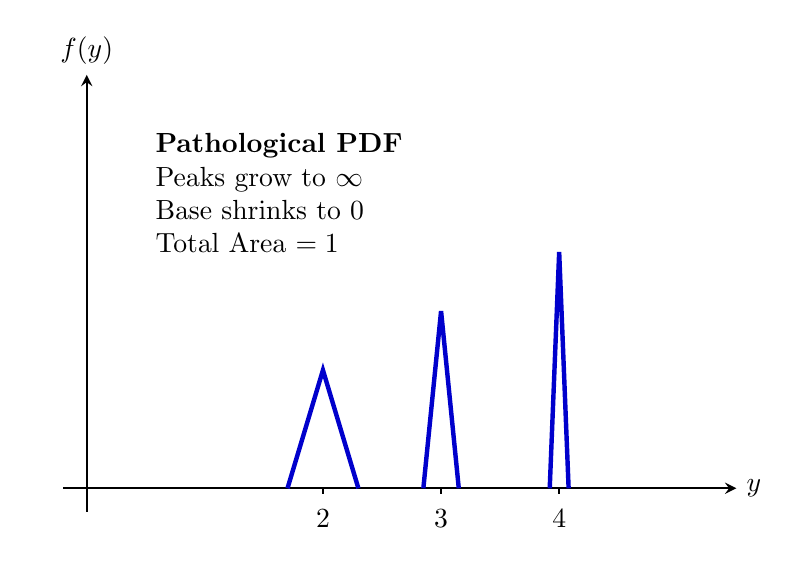
\begin{tikzpicture}[scale=1.5]
    \fill[white] (-0.5,-0.5) rectangle (5.5, 3.5);
    \draw[thick, ->, >=stealth] (-0.2,0) -- (5.5,0) node[right] {$y$};
    \draw[thick, ->, >=stealth] (0,-0.2) -- (0,3.5) node[above] {$f(y)$};
    
    % Tent 1 (n=2)
    \draw[ultra thick, blue!80!black] (1.7,0) -- (2, 1) -- (2.3, 0);
    \draw[thick] (2,0) -- (2,-0.05) node[below=2pt] {$2$};
    
    % Tent 2 (n=3)
    \draw[ultra thick, blue!80!black] (2.85,0) -- (3, 1.5) -- (3.15, 0);
    \draw[thick] (3,0) -- (3,-0.05) node[below=2pt] {$3$};
    
    % Tent 3 (n=4)
    \draw[ultra thick, blue!80!black] (3.92,0) -- (4, 2) -- (4.08, 0);
    \draw[thick] (4,0) -- (4,-0.05) node[below=2pt] {$4$};
    
    \node[align=left, anchor=west, black] at (0.5, 2.5) {
        \textbf{Pathological PDF}\\
        Peaks grow to $\infty$\\
        Base shrinks to $0$\\
        Total Area $= 1$
    };
\end{tikzpicture}
\end{proof}

\textbf{Solution 5:}
\begin{proof}
The set of rational numbers $\Q$ is countably infinite. Therefore, it can be enumerated as a sequence $\{q_1, q_2, q_3, \dots\}$.
By the countable additivity axiom of probability measures (Kolmogorov's Third Axiom):
\[ \Prob(Y \in \Q) = \Prob\left(\bigcup_{i=1}^\infty \{Y = q_i\}\right) = \sum_{i=1}^\infty \Prob(Y = q_i) \]
Since $Y$ is a continuous random variable, the probability of it taking any exact value is zero, meaning $\Prob(Y = q_i) = 0$ for all $i$.
\[ \Prob(Y \in \Q) = \sum_{i=1}^\infty 0 = 0 \]
\end{proof}

\subsection{CDF/PDF Conversions and Quantiles}

\textbf{Solution 6:}
\begin{proof}
The median $m$ is defined as the value such that $F(m) = 0.5$. 
If $F(y)$ is strictly increasing, it is a bijective function on its support. Therefore, its inverse $F^{-1}$ exists and is single-valued. Thus, $m = F^{-1}(0.5)$ is unique.
If $F(y)$ is constant over an interval $[a, b]$ such that $F(y) = 0.5$ for all $y \in [a, b]$, then any value $m \in [a, b]$ satisfies the definition of the median. Hence, the median is not unique.
\end{proof}

\textbf{Solution 7:}
\begin{proof}
First, we find the CDF $F(y)$ by integrating the PDF:
\[ F(y) = \int_{y_m}^y \alpha y_m^\alpha t^{-\alpha-1} dt = \alpha y_m^\alpha \left[ \frac{t^{-\alpha}}{-\alpha} \right]_{y_m}^y = -y_m^\alpha (y^{-\alpha} - y_m^{-\alpha}) = 1 - \left(\frac{y_m}{y}\right)^\alpha \]
The $p$-th quantile $\phi_p$ is the value such that $F(\phi_p) = p$:
\[ 1 - \left(\frac{y_m}{\phi_p}\right)^\alpha = p \implies \left(\frac{y_m}{\phi_p}\right)^\alpha = 1 - p \implies \frac{y_m}{\phi_p} = (1-p)^{1/\alpha} \]
Solving for $\phi_p$:
\[ \phi_p = \frac{y_m}{(1-p)^{1/\alpha}} \]
\end{proof}

\textbf{Solution 8:}
\begin{proof}
Let $U = F(Y)$. Since $F$ is a CDF, $0 \le U \le 1$. We want to find the CDF of $U$, denoted $F_U(u) = \Prob(U \le u)$.
For $u \in [0,1]$:
\[ F_U(u) = \Prob(F(Y) \le u) \]
Since $F$ is strictly increasing, its inverse $F^{-1}$ exists and is strictly increasing. We apply $F^{-1}$ to both sides of the inequality:
\[ F_U(u) = \Prob(Y \le F^{-1}(u)) \]
By the definition of the CDF of $Y$:
\[ \Prob(Y \le F^{-1}(u)) = F(F^{-1}(u)) = u \]
Thus, $F_U(u) = u$ for $u \in [0,1]$, which is exactly the CDF of a Uniform(0,1) distribution.
\end{proof}

\textbf{Solution 9:}
\begin{proof}
The flaw is confusing the properties of the PDF with the CDF. The PDF integrates to 1: $\int_{-\infty}^\infty f(y) dy = 1$. 
The CDF $F(y)$ represents cumulative probability, meaning $\lim_{y \to \infty} F(y) = 1$. 
When evaluating the integral of the CDF over the real line:
\[ \int_{-\infty}^\infty F(y) dy = \int_{-\infty}^0 F(y) dy + \int_0^\infty F(y) dy \]
Since $\lim_{y \to \infty} F(y) = 1$, for sufficiently large $y$, $F(y)$ is arbitrarily close to 1. Integrating a constant 1 over an infinite interval $[M, \infty)$ yields infinity. Therefore, the integral strictly diverges.
\end{proof}

\textbf{Solution 10:}
\begin{proof}
The survival function is $S(y) = 1 - F(y)$. Therefore, the CDF is $F(y) = 1 - S(y) = 1 - e^{-\lambda y^2}$.
To find the PDF $f(y)$, we differentiate the CDF with respect to $y$:
\[ f(y) = \frac{d}{dy} \left( 1 - e^{-\lambda y^2} \right) = -e^{-\lambda y^2} \cdot \frac{d}{dy}(-\lambda y^2) = -e^{-\lambda y^2} \cdot (-2\lambda y) = 2\lambda y e^{-\lambda y^2} \]
for $y \ge 0$.
\end{proof}

\subsection{Moments, LOTUS, and Variance}

\textbf{Solution 11:}
\begin{proof}
By definition, $E[g(Y)] = \int_{-\infty}^\infty g(y)f(y) dy$. Let $g(Y) = aY + b$.
\[ E[aY+b] = \int_{-\infty}^\infty (ay+b)f(y) dy \]
Using the linearity of the Lebesgue integral:
\[ = \int_{-\infty}^\infty ay f(y) dy + \int_{-\infty}^\infty b f(y) dy = a \int_{-\infty}^\infty y f(y) dy + b \int_{-\infty}^\infty f(y) dy \]
Since $\int_{-\infty}^\infty y f(y) dy = E[Y]$ and $\int_{-\infty}^\infty f(y) dy = 1$:
\[ E[aY+b] = aE[Y] + b(1) = aE[Y] + b \]
\end{proof}

\textbf{Solution 12:}
\begin{proof}
Consider a random variable $Y$ with a Pareto-like PDF $f(y) = \frac{2}{y^3}$ for $y \ge 1$, and $0$ elsewhere.
The first moment is:
\[ E[Y] = \int_1^\infty y \left(\frac{2}{y^3}\right) dy = \int_1^\infty \frac{2}{y^2} dy = \left[ -\frac{2}{y} \right]_1^\infty = 0 - (-2) = 2 \]
The first moment exists and is finite. Now consider the second moment:
\[ E[Y^2] = \int_1^\infty y^2 \left(\frac{2}{y^3}\right) dy = \int_1^\infty \frac{2}{y} dy = \left[ 2 \ln(y) \right]_1^\infty \to \infty \]
The integral diverges. Thus, the existence of $E[Y]$ does not guarantee the existence of $E[Y^2]$.
\end{proof}

\textbf{Solution 13:}
\begin{proof}
By definition, $V(Y) = E[(Y - \mu)^2]$ where $\mu = E[Y]$. 
Since $(Y - \mu)^2 \ge 0$ for all $Y \in \R$, its expected value (the integral of a non-negative function multiplied by a non-negative PDF) must be non-negative. Thus, $V(Y) \ge 0$.
Expanding the square:
\[ V(Y) = E[Y^2 - 2\mu Y + \mu^2] = E[Y^2] - 2\mu E[Y] + \mu^2 = E[Y^2] - 2\mu^2 + \mu^2 = E[Y^2] - \mu^2 \]
$V(Y) = 0$ if and only if $E[(Y - \mu)^2] = 0$. Since the integrand $(y-\mu)^2 f(y)$ is non-negative, the integral is zero if and only if $(y-\mu)^2 f(y) = 0$ almost everywhere. This implies $Y = \mu$ with probability 1, meaning $Y$ is a degenerate (constant) random variable.
\end{proof}

\textbf{Solution 14:}
\begin{proof}
The PDF is $f(y) = \frac{1}{2} e^{-|y|}$. The expected value is:
\[ E[Y] = \int_{-\infty}^\infty y \left(\frac{1}{2} e^{-|y|}\right) dy \]
Notice that $g(y) = y$ is an odd function ($g(-y) = -g(y)$), and $f(y) = \frac{1}{2} e^{-|y|}$ is an even function ($f(-y) = f(y)$). 
The product of an odd function and an even function is an odd function. 
The integral of an odd function over a symmetric interval $(-\infty, \infty)$ is $0$, provided the integral of the absolute value converges.
Checking convergence: $\int_0^\infty y e^{-y} dy = 1 < \infty$. 
Therefore, $E[Y] = 0$.
\end{proof}

\textbf{Solution 15:}
\begin{proof}
This is identical in structure to Solution 11, reinforcing the foundational axiom of integral linearity.
\[ E[aY+b] = \int_{-\infty}^\infty (ay+b)f(y) dy = a \int_{-\infty}^\infty y f(y) dy + b \int_{-\infty}^\infty f(y) dy = aE[Y] + b \]
\end{proof}

\subsection{Advanced Proofs and Fubini-Tonelli}

\textbf{Solution 16:}
\begin{proof}
We start with the right-hand side. By definition, $1 - F(y) = \Prob(Y > y) = \int_y^\infty f(t) dt$.
\[ \int_0^\infty [1 - F(y)] dy = \int_0^\infty \left( \int_y^\infty f(t) dt \right) dy \]
This is a double integral over the region $0 \le y \le t < \infty$. Since $f(t) \ge 0$, we can apply the Tonelli-Fubini Theorem to reverse the order of integration. 
The bounds change to $t$ ranging from $0$ to $\infty$, and for a fixed $t$, $y$ ranges from $0$ to $t$:
\[ = \int_0^\infty \left( \int_0^t f(t) dy \right) dt \]
Since $f(t)$ is constant with respect to $y$, we pull it out of the inner integral:
\[ = \int_0^\infty f(t) \left( \int_0^t 1 dy \right) dt = \int_0^\infty f(t) [y]_0^t dt = \int_0^\infty t f(t) dt \]
By definition, this final integral is exactly $E[Y]$.

\vspace{10pt}
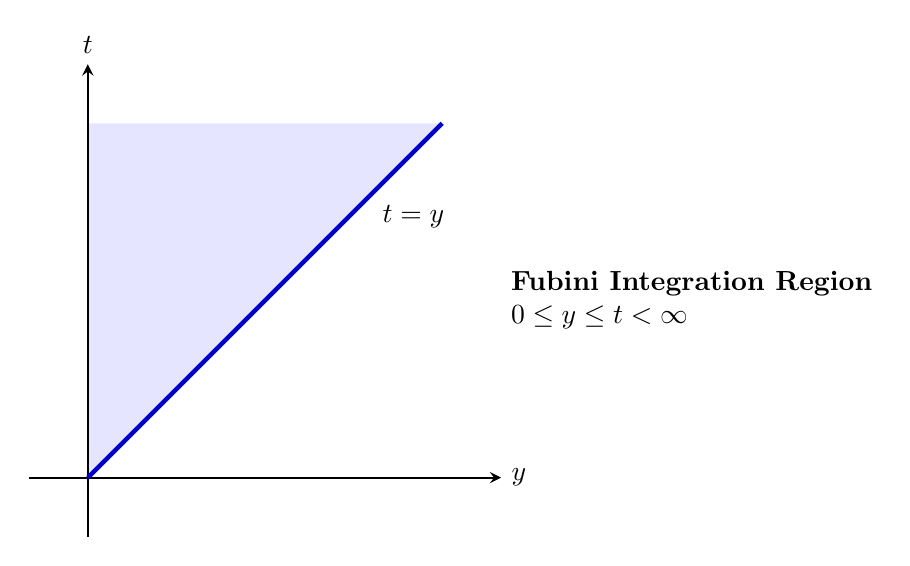
\begin{tikzpicture}[scale=1.5]
    \fill[blue!10] (0,0) -- (3,3) -- (0,3) -- cycle;
    \draw[thick, ->, >=stealth] (-0.5,0) -- (3.5,0) node[right] {$y$};
    \draw[thick, ->, >=stealth] (0,-0.5) -- (0,3.5) node[above] {$t$};
    \draw[ultra thick, blue!80!black] (0,0) -- (3,3) node[pos=0.8, below right, black] {$t = y$};
    \node[align=left, anchor=west, black] at (3.5, 1.5) {
        \textbf{Fubini Integration Region}\\
        $0 \le y \le t < \infty$
    };
\end{tikzpicture}
\end{proof}

\textbf{Solution 17:}
\begin{proof}
We evaluate the right-hand side:
\[ 2 \int_0^\infty y [1 - F(y)] dy = 2 \int_0^\infty y \left( \int_y^\infty f(t) dt \right) dy \]
Using Fubini's Theorem to swap the order of integration over the region $0 \le y \le t < \infty$:
\[ = 2 \int_0^\infty \left( \int_0^t y f(t) dy \right) dt = 2 \int_0^\infty f(t) \left( \int_0^t y dy \right) dt \]
Evaluate the inner integral:
\[ \int_0^t y dy = \left[ \frac{y^2}{2} \right]_0^t = \frac{t^2}{2} \]
Substitute this back:
\[ = 2 \int_0^\infty f(t) \left( \frac{t^2}{2} \right) dt = \int_0^\infty t^2 f(t) dt = E[Y^2] \]
\end{proof}

\textbf{Solution 18:}
\begin{proof}
Let $I$ be an indicator function such that $I = 1$ if $|Y-\mu| \ge k\sigma$, and $I = 0$ otherwise.
Notice that for all $Y$, the following inequality holds:
\[ I \le \frac{(Y-\mu)^2}{k^2\sigma^2} \]
If $|Y-\mu| < k\sigma$, $I=0$, and the right side is $\ge 0$. If $|Y-\mu| \ge k\sigma$, $I=1$, and the right side is $\ge 1$.
Taking the expectation of both sides (expectation preserves inequalities):
\[ E[I] \le E\left[ \frac{(Y-\mu)^2}{k^2\sigma^2} \right] \]
The expectation of an indicator function is the probability of the event: $E[I] = \Prob(|Y-\mu| \ge k\sigma)$.
By linearity of expectation:
\[ \Prob(|Y-\mu| \ge k\sigma) \le \frac{1}{k^2\sigma^2} E[(Y-\mu)^2] \]
Since $E[(Y-\mu)^2] = \sigma^2$:
\[ \Prob(|Y-\mu| \ge k\sigma) \le \frac{\sigma^2}{k^2\sigma^2} = \frac{1}{k^2} \]
\end{proof}

\textbf{Solution 19:}
\begin{proof}
We expand the expectation on the right-hand side:
\[ \frac{1}{2} E[(Y_1 - Y_2)^2] = \frac{1}{2} E[Y_1^2 - 2Y_1Y_2 + Y_2^2] \]
Using linearity of expectation:
\[ = \frac{1}{2} \left( E[Y_1^2] - 2E[Y_1Y_2] + E[Y_2^2] \right) \]
Since $Y_1$ and $Y_2$ are identically distributed copies of $Y$, $E[Y_1^2] = E[Y_2^2] = E[Y^2]$ and $E[Y_1] = E[Y_2] = E[Y]$.
Since they are independent, $E[Y_1Y_2] = E[Y_1]E[Y_2] = (E[Y])^2$.
Substitute these in:
\[ = \frac{1}{2} \left( E[Y^2] - 2(E[Y])^2 + E[Y^2] \right) = \frac{1}{2} \left( 2E[Y^2] - 2(E[Y])^2 \right) = E[Y^2] - (E[Y])^2 = V(Y) \]
\end{proof}

\textbf{Solution 20:}
\begin{proof}
The fallacy assumes variance is a linear operator. Let $X$ and $Y$ be independent random variables.
\[ V(X-Y) = V(X + (-Y)) \]
By the definition of variance for independent variables, $V(A+B) = V(A) + V(B)$.
\[ V(X-Y) = V(X) + V(-Y) \]
Using the variance scaling property $V(aY) = a^2V(Y)$ with $a = -1$:
\[ V(-Y) = (-1)^2 V(Y) = V(Y) \]
Therefore, $V(X-Y) = V(X) + V(Y)$. Variances of independent variables always add, even when the variables are subtracted.
\end{proof}

\subsection{Transformations (The Jacobian Method)}

\textbf{Solution 21:}
\begin{proof}
Let $Y \sim N(0,1)$ with PDF $f_Y(y) = \frac{1}{\sqrt{2\pi}} e^{-y^2/2}$. We want the PDF of $U = Y^2$.
First, find the CDF of $U$, $F_U(u) = \Prob(U \le u)$. Since $U = Y^2 \ge 0$, $F_U(u) = 0$ for $u < 0$.
For $u \ge 0$:
\[ F_U(u) = \Prob(Y^2 \le u) = \Prob(-\sqrt{u} \le Y \le \sqrt{u}) = F_Y(\sqrt{u}) - F_Y(-\sqrt{u}) \]
Differentiate with respect to $u$ using the Chain Rule to find the PDF $f_U(u)$:
\[ f_U(u) = \frac{d}{du} \left[ F_Y(\sqrt{u}) - F_Y(-\sqrt{u}) \right] = f_Y(\sqrt{u}) \cdot \frac{1}{2\sqrt{u}} - f_Y(-\sqrt{u}) \cdot \left(-\frac{1}{2\sqrt{u}}\right) \]
Since the standard normal PDF is symmetric, $f_Y(\sqrt{u}) = f_Y(-\sqrt{u})$:
\[ f_U(u) = \frac{1}{2\sqrt{u}} f_Y(\sqrt{u}) + \frac{1}{2\sqrt{u}} f_Y(\sqrt{u}) = \frac{1}{\sqrt{u}} f_Y(\sqrt{u}) \]
Substitute the normal PDF:
\[ f_U(u) = \frac{1}{\sqrt{u}} \frac{1}{\sqrt{2\pi}} e^{-(\sqrt{u})^2/2} = \frac{1}{\sqrt{2\pi u}} e^{-u/2} \quad \text{for } u > 0 \]
This is the PDF of a Chi-Square distribution with 1 degree of freedom.
\end{proof}

\textbf{Solution 22:}
\begin{proof}
Consider a Uniform distribution on the interval $[0, 0.01]$. 
The PDF is $f(y) = \frac{1}{b-a} = \frac{1}{0.01 - 0} = 100$ for $y \in [0, 0.01]$, and $0$ elsewhere.
Here, $f(0) = 100$, which is strictly greater than 1. 
This is perfectly valid because the PDF represents probability \textit{density}, not probability itself. The integral over the support is $\int_0^{0.01} 100 dy = 100(0.01) = 1$, satisfying the axioms.
\end{proof}

\textbf{Solution 23:}
\begin{proof}
Let $Y \sim \text{Uniform}(0,1)$, so $f_Y(y) = 1$ for $y \in [0,1]$. Let $U = -\frac{1}{\lambda} \ln(Y)$.
The transformation $g(y) = -\frac{1}{\lambda} \ln(y)$ is strictly monotonically decreasing on $(0,1)$.
We use the Jacobian method. The inverse transformation is $y = g^{-1}(u) = e^{-\lambda u}$.
The derivative is $\frac{dy}{du} = -\lambda e^{-\lambda u}$.
The PDF of $U$ is:
\[ f_U(u) = f_Y(g^{-1}(u)) \left| \frac{dy}{du} \right| = 1 \cdot \left| -\lambda e^{-\lambda u} \right| = \lambda e^{-\lambda u} \]
Since $y \in (0,1)$, $u \in (0, \infty)$. Thus, $U$ follows an Exponential distribution with rate $\lambda$.
\end{proof}

\textbf{Solution 24:}
\begin{proof}
The Jacobian method $f_U(u) = f_Y(g^{-1}(u)) \left| \frac{d}{du} g^{-1}(u) \right|$ strictly requires the transformation $g(y)$ to be monotonic (either strictly increasing or strictly decreasing) over the entire support of $Y$. 
The function $g(y) = \sin(y)$ is not monotonic over $\R$; it oscillates. Therefore, $g^{-1}(u)$ is not a single-valued function (it has infinitely many branches). Applying the formula blindly ignores the probability mass contributed by all the other branches of the inverse, leading to an incorrect, unnormalized PDF.
\end{proof}

\textbf{Solution 25:}
\begin{proof}
Let $U = |Y|$. The CDF of $U$ for $u \ge 0$ is:
\[ F_U(u) = \Prob(|Y| \le u) = \Prob(-u \le Y \le u) = F_Y(u) - F_Y(-u) \]
Differentiating with respect to $u$:
\[ f_U(u) = f_Y(u) - f_Y(-u) \cdot (-1) = f_Y(u) + f_Y(-u) \]
Since $f_Y(y)$ is symmetric around $0$, $f_Y(-u) = f_Y(u)$.
\[ f_U(u) = 2f_Y(u) \quad \text{for } u \ge 0 \]
\end{proof}

\subsection{Abstract Real-World Modeling \& Synthesis}

\textbf{Solution 26:}
\begin{proof}
The payoff of the call option is $\max(S_T - K, 0)$. If $K=0$, the payoff is simply $S_T$.
We need to evaluate $E^\Q[S_T]$. Under the risk-neutral measure, $S_T = S_0 e^{(r-\sigma^2/2)T + \sigma \sqrt{T} Z}$ where $Z \sim N(0,1)$.
\[ E^\Q[S_T] = E^\Q\left[ S_0 e^{(r-\sigma^2/2)T} e^{\sigma \sqrt{T} Z} \right] \]
Since $S_0$ and $e^{(r-\sigma^2/2)T}$ are constants, we pull them out:
\[ = S_0 e^{(r-\sigma^2/2)T} E^\Q\left[ e^{\sigma \sqrt{T} Z} \right] \]
The term $E^\Q[e^{\sigma \sqrt{T} Z}]$ is the Moment Generating Function (MGF) of a standard normal variable $Z$, evaluated at $t = \sigma \sqrt{T}$. The MGF of $N(0,1)$ is $M_Z(t) = e^{t^2/2}$.
\[ E^\Q\left[ e^{\sigma \sqrt{T} Z} \right] = e^{(\sigma \sqrt{T})^2 / 2} = e^{\sigma^2 T / 2} \]
Substitute this back:
\[ E^\Q[S_T] = S_0 e^{(r-\sigma^2/2)T} e^{\sigma^2 T / 2} = S_0 e^{rT - \sigma^2 T / 2 + \sigma^2 T / 2} = S_0 e^{rT} \]
\end{proof}

\textbf{Solution 27:}
\begin{proof}
Building directly on the result from Solution 26, we established that $E^\Q[S_T] = S_0 e^{rT}$.
The Fundamental Theorem of Asset Pricing states the price today is the discounted expected payoff:
\[ C_0 = e^{-rT} E^\Q[S_T] = e^{-rT} (S_0 e^{rT}) = S_0 e^{-rT + rT} = S_0 \]
This proves that under the risk-neutral measure, the discounted stock price is a martingale.
\end{proof}

\textbf{Solution 28:}
\begin{proof}
The KL divergence is defined as $D_{KL}(P \parallel Q) = \int_0^\infty p(y) \ln\left(\frac{p(y)}{q(y)}\right) dy$.
Given $p(y) = \lambda_1 e^{-\lambda_1 y}$ and $q(y) = \lambda_2 e^{-\lambda_2 y}$:
\[ \ln\left(\frac{p(y)}{q(y)}\right) = \ln\left(\frac{\lambda_1 e^{-\lambda_1 y}}{\lambda_2 e^{-\lambda_2 y}}\right) = \ln\left(\frac{\lambda_1}{\lambda_2}\right) - \lambda_1 y + \lambda_2 y = \ln\left(\frac{\lambda_1}{\lambda_2}\right) - (\lambda_1 - \lambda_2)y \]
Substitute this into the integral:
\[ D_{KL}(P \parallel Q) = \int_0^\infty \lambda_1 e^{-\lambda_1 y} \left[ \ln\left(\frac{\lambda_1}{\lambda_2}\right) - (\lambda_1 - \lambda_2)y \right] dy \]
Split the integral:
\[ = \ln\left(\frac{\lambda_1}{\lambda_2}\right) \int_0^\infty \lambda_1 e^{-\lambda_1 y} dy - (\lambda_1 - \lambda_2) \int_0^\infty y \lambda_1 e^{-\lambda_1 y} dy \]
The first integral is the integral of a PDF, which equals 1. The second integral is the expected value of $P$, which is $1/\lambda_1$.
\[ D_{KL}(P \parallel Q) = \ln\left(\frac{\lambda_1}{\lambda_2}\right) - (\lambda_1 - \lambda_2)\left(\frac{1}{\lambda_1}\right) = \ln\left(\frac{\lambda_1}{\lambda_2}\right) - 1 + \frac{\lambda_2}{\lambda_1} \]
\end{proof}

\textbf{Solution 29:}
\begin{proof}
Jensen's Inequality states that for any convex function $g(y)$ and random variable $Y$, $E[g(Y)] \ge g(E[Y])$.
Let $g(y) = 1/y$ for $y > 0$. We check for convexity by finding the second derivative:
\[ g'(y) = -y^{-2}, \quad g''(y) = 2y^{-3} \]
Since $y > 0$, $g''(y) > 0$, meaning $g(y)$ is strictly convex.
By Jensen's Inequality:
\[ E\left[\frac{1}{Y}\right] \ge \frac{1}{E[Y]} \]
Because $g(y)$ is strictly convex, the inequality is strict ($>$) unless $Y$ is a degenerate constant. Therefore, the claim $E[1/Y] = 1/E[Y]$ is mathematically false.
\end{proof}

\textbf{Solution 30:}
\begin{proof}
We are given the hazard rate $h(y) = \frac{f(y)}{1-F(y)} = \lambda$.
Notice that $f(y) = \frac{d}{dy} F(y) = -\frac{d}{dy} (1-F(y))$.
Substitute this into the hazard rate equation:
\[ \frac{-\frac{d}{dy} (1-F(y))}{1-F(y)} = \lambda \]
Integrate both sides with respect to $y$:
\[ \int \frac{-\frac{d}{dy} (1-F(y))}{1-F(y)} dy = \int \lambda dy \]
\[ -\ln(1-F(y)) = \lambda y + C \]
Since $Y$ is a time to failure, $Y \ge 0$, so $F(0) = 0$.
\[ -\ln(1-0) = \lambda(0) + C \implies -\ln(1) = C \implies C = 0 \]
Thus, $-\ln(1-F(y)) = \lambda y \implies 1-F(y) = e^{-\lambda y} \implies F(y) = 1 - e^{-\lambda y}$.
This is the exact CDF of an Exponential distribution.
\end{proof}

\newpage

\section{Concept Checklist \& Question Mapping (Reference)}
\label{sec:checklist_end}

\renewcommand{\arraystretch}{1.5}
\noindent
\begin{tabularx}{\textwidth}{>{\bfseries}l X c}
\toprule
ID & Concept / Proof Technique & Problem Mapping \\
\midrule
C1 & Measure-Theoretic Foundations \& PDF Axioms & 1, 3, 5 \\
C2 & Pathological Counterexamples (PDF $> 1$, Divergence) & 2, 4, 9, 22 \\
C3 & CDF-PDF Conversions \& Quantile Derivations & 6, 7, 10 \\
C4 & Probability Integral Transform (PIT) & 8 \\
C5 & Moments, LOTUS, and Integration by Parts & 11, 12, 14, 15 \\
C6 & Variance Properties \& Linearity Fallacies & 13, 19, 20, 24 \\
C7 & Fubini-Tonelli Theorem (Swapping Integrals) & 16, 17, 27 \\
C8 & Indicator Functions \& Chebyshev's Inequality & 18 \\
C9 & Transformations of Variables (Jacobian Method) & 21, 23, 25 \\
C10 & Abstract Modeling: Quantitative Finance (Black-Scholes) & 26, 27 \\
C11 & Abstract Modeling: Generative AI (KL Divergence) & 28 \\
C12 & Advanced Diagnostic Testing (Jensen's Inequality) & 29 \\
C13 & Hazard Rates and Distributional Characterizations & 30 \\
\bottomrule
\end{tabularx}

\end{document}